\documentclass[tikz,border=3.14mm]{standalone}
\usetikzlibrary{shapes,arrows,positioning}

\begin{document}
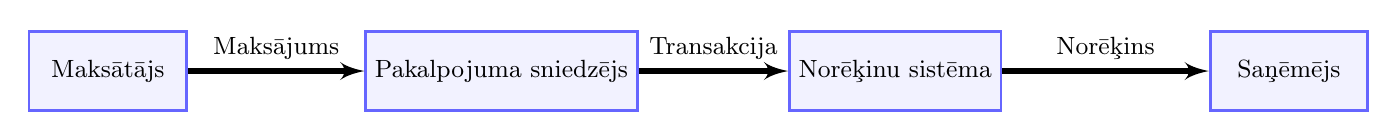
\begin{tikzpicture}[
    block/.style={rectangle, draw=blue!60, fill=blue!5, line width=1pt, minimum width=2cm, minimum height=1cm, text centered},
    arrow/.style={draw, -latex', line width=2pt},
    node distance=5cm
]

  \tikzset{
    font={\fontsize{9pt}{12}\selectfont}
  }
% Nodes
\node[block] (payer) {Maksātājs};
\node[block, right of=payer] (paymentprovider) {Pakalpojuma sniedzējs};
\node[block, right of=paymentprovider] (settlementsystem) {Norēķinu sistēma};
\node[block, right of=settlementsystem] (payee) {Saņēmējs};

% Lines
\draw[arrow] (payer) -- node[above] {Maksājums} (paymentprovider);
\draw[arrow] (paymentprovider) -- node[above] {Transakcija} (settlementsystem);
\draw[arrow] (settlementsystem) -- node[above] {Norēķins} (payee);

\end{tikzpicture}
\end{document}
